\clearpage
\section{Results}
\label{sec:results}

\subsection{The agents did not produce research at the caliber of a top ML
conference}

We asked the authors of the two papers to review the agents' outputs in depth.
Alongside their qualitative review, we asked them to score the paper on a scale
of 1 (``Strong Reject'') to 6 (``Strong Accept''), mirroring official reviews
at AI conferences.

The authors rejected both papers. The Personas paper was scored a 2
(``Reject''), and the TabPFN paper was scored a 1 (``Strong Reject''). Both
reviews highlighted the same failures: poorly motivated data and experiments,
no novel contribution, and impenetrable prose.

\begin{itemize}[leftmargin=*,itemsep=3pt]
  \item ``The experiments and methodological choices were bizarre, and hard
  to understand. The results seem clearly a result of post hoc choices,''
  David Africa wrote.
  \item Viet Nguyen flagged the poor reasoning of the agent: ``Upon testing a
  few unsuccessful signals using a PFN's internals, going from there to
  `there are no signals we can use that leverage a model's internals' is a huge
  leap, a kind of `proof by example' fallacy that is highly non-scientific.''
  \item Both flagged the poor writing. Nguyen: ``impossible to quickly distill
  what is noise and what is important.'' Africa: ``dense and heavily hedged,
  often to the point of obscuring what was actually done and found.''
\end{itemize}

Our survey respondents assigned a median probability of a weak accept or better of
30\%. Most of them expected failure for the same reasons highlighted by the
reviewers: the lack of creativity and judgment.

\subsection{The agents produced a small number of findings that interested the
authors of the original papers}

Both authors were impressed with the literature review and the fact that the
agents were able to utilize hundreds of GPU hours on real experiments without
issue. Both noted that the candidate hypotheses were similar to their own
initial approaches to the problem. While they did not substantively answer the
research questions, the agents did produce minor findings that were noted as
relevant by reviewers.\footnote{In the Personas paper, the agent produced a potentially interesting counterintuitive result. In emergent misalignment, narrow finetuning on harmful or risky responses can generalise broadly. The agent found that narrow finetuning on only the misaligned style did not translate to broad misgeneralisation.} Respondents had given a median 60\% chance that the agents
would meet this more moderate criterion.

\begin{figure}[p]
  \centering
  % Full-width stacked panels keep the three resource traces and annotations
% legible at normal page size.
\textbf{\headingfont Personas}\par\smallskip
{\small\headingfont\bfseries\color{cruxink}
In the Personas run, the agent used just over a third of the available token
budget.\par}
\smallskip

\begin{tikzpicture}
\begin{axis}[
  resource timeline,
  width=0.95\linewidth,
  height=0.32\linewidth,
  legend columns=3,
  legend style={
    at={(0.5,1.25)},anchor=south,draw=none,fill=none,
    font=\scriptsize\headingfont\bfseries,
    /tikz/every even column/.append style={column sep=1.0em}
  }
]
  \TimelineMarker{1}{14}
  \TimelineMarker{2}{51}
  \TimelineMarker{3}{84}
  \TimelineMarker{4}{104}
  \TimelineMarker{5}{118.8}
  \TimelineMarker{6}{137}
  \TimelineDeadline[118.8]

  \TimelineWallClockPlot{
    (0,0) (6,5) (12,10.1) (18,15.1) (24,20.2) (30,25.2)
    (36,30.3) (42,35.3) (48,40.4) (54,45.4) (60,50.5)
    (66,55.5) (72,60.6) (78,65.6) (84,70.7) (90,75.7)
    (96,80.8) (102,85.8) (108,90.9) (114,95.9) (118.8,100)
    (119,83.5) (120,84.3) (126,88.5) (132,92.7) (138,96.9)
    (142.4,100)
  }

  \addplot+[draw=timelineapi,line width=1.45pt,mark=*,mark size=1.4pt,
            mark options={fill=timelineapi,draw=timelineapi}]
    coordinates {
      (0,0) (6,3.0) (12,4.2) (18,6.5) (24,8.2) (30,9.5)
      (36,10.3) (42,11.4) (48,11.7) (54,12.2) (60,12.4)
      (66,12.6) (72,12.7) (78,13.1) (84,15.2) (90,16.7)
      (96,17.6) (102,20.8) (108,21.8) (114,24.0) (118.8,27.8)
      (119,28.0) (120,28.9) (126,30.9) (132,32.8) (138,35.3)
      (142.4,37.7)
    };
  \addlegendentry{Anthropic API spend}

  \addplot+[draw=timelinegpu,line width=1.45pt,mark=*,mark size=1.4pt,
            mark options={fill=timelinegpu,draw=timelinegpu}]
    coordinates {
      (0,0) (6,0.2) (12,1.6) (18,3.8) (24,6.5) (30,8.2)
      (36,10.9) (42,14.4) (48,19.5) (54,23.6) (60,26.9)
      (66,30.3) (72,33.7) (78,36.8) (84,38.4) (90,42.1)
      (96,44.5) (102,49.2) (108,58.9) (114,64.2) (118.8,65.0)
      (119,65.0) (120,65.5) (126,69.7) (132,74.2) (138,78.4)
      (142.4,78.4)
    };
  \addlegendentry{GPU compute}

  \node[timeline value label,anchor=north east,
        draw=timelineapi!45,text=timelineapi] (personas-api-value)
    at (axis cs:142.4,22.0) {\$1,130 of \$3,000};
  \draw[timelineapi,line width=0.7pt]
    (axis cs:142.4,37.7) -- (personas-api-value.north);
  \node[timeline value label,anchor=north east,
        draw=timelinegpu!45,text=timelinegpu] (personas-gpu-value)
    at (axis cs:142.4,62.0) {\$392 of \$500};
  \draw[timelinegpu,line width=0.7pt]
    (axis cs:142.4,78.4) -- (personas-gpu-value.north);
\end{axis}
\end{tikzpicture}

\centering\TimelineExtensionKey

\smallskip
{\scriptsize\headingfont
\begin{minipage}[t]{0.485\linewidth}
\renewcommand{\arraystretch}{1.10}
\begin{tabularx}{\linewidth}{@{}p{5.5mm}Y@{}}
  \TimelineEventText{1}{The agent retires its planned headline finding --- a
    positive claim showing traits transferring to untrained behaviors --- after
    an early test produces a null result.}
  \TimelineEventText{2}{The agent rapidly scales up the compute for its negative
    finding, showing it replicates on Qwen models from 3B to 14B parameters
    ($\sim$7 GPU-hours per seed) and on Llama-3.}
  \TimelineEventText{3}{The agent's first blind review returns a 3/10 reject, so
    it runs a series of stronger follow-up experiments that the reviewer
    demands.}
\end{tabularx}
\end{minipage}\hfill
\begin{minipage}[t]{0.485\linewidth}
\renewcommand{\arraystretch}{1.10}
\begin{tabularx}{\linewidth}{@{}p{5.5mm}Y@{}}
  \TimelineEventText{4}{The agent runs a test on a rival steering method on
    three A100s with an identical training budget, which overturns the paper's
    headline claim.}
  \TimelineEventText{5}{The agent reports completion; the paper is finished but
    self-graded below the Weak Accept bar. A 24-hour extension is granted.}
  \TimelineEventText{6}{The agent makes a final bet on a nine-hour three-A100
    test of a new method, which fails decisively; the agent logs the negative
    result and concludes.}
\end{tabularx}
\end{minipage}
}

%\medskip
%\hrule height 0.35pt
%\medskip

\bigskip

\textbf{\headingfont TabPFN}\par\smallskip
{\small\headingfont\bfseries\color{cruxink}
In the TabPFN run, the agent used only 40\% of the available token budget.\par}
\smallskip

\begin{tikzpicture}
\begin{axis}[
  resource timeline,
  width=0.95\linewidth,
  height=0.32\linewidth,
  legend columns=3,
  legend style={
    at={(0.5,1.25)},anchor=south,draw=none,fill=none,
    font=\scriptsize\headingfont\bfseries,
    /tikz/every even column/.append style={column sep=1.0em}
  }
]
  \TimelineMarker{1}{10}
  \TimelineMarker{2}{23}
  \TimelineMarker{3}{47}
  \TimelineMarker{4}{94}
  \TimelineMarker{5}{119}
  \TimelineMarker{6}{142.5}
  \TimelineDeadline[119]

  \TimelineWallClockPlot{
    (0,0) (6,5) (12,10.1) (18,15.1) (24,20.2) (30,25.2)
    (36,30.3) (42,35.3) (48,40.4) (54,45.4) (60,50.4)
    (66,55.5) (72,60.5) (78,65.6) (84,70.6) (90,75.7)
    (96,80.7) (102,85.8) (108,90.8) (114,95.8) (119,100)
    (119,83.5) (120,84.2) (126,88.4) (132,92.6) (138,96.8)
    (142.5,100)
  }

  \addplot+[draw=timelineapi,line width=1.45pt,mark=*,mark size=1.4pt,
            mark options={fill=timelineapi,draw=timelineapi}]
    coordinates {
      (0,0) (6,3.6) (12,6.1) (18,6.8) (24,8.4) (30,8.9)
      (36,9.7) (42,11.0) (48,15.7) (54,19.3) (60,20.0)
      (66,20.5) (72,20.9) (78,21.2) (84,21.9) (90,24.9)
      (96,25.4) (102,25.8) (108,26.3) (114,27.7) (119,29.8)
      (119,29.9) (120,30.7) (126,31.8) (132,34.8) (138,38.8)
      (142.5,41.2)
    };
  \addlegendentry{Anthropic API spend}

  \addplot+[draw=timelinegpu,line width=1.45pt,mark=*,mark size=1.4pt,
            mark options={fill=timelinegpu,draw=timelinegpu}]
    coordinates {
      (0,0) (6,0) (12,0) (18,0) (24,1.3) (30,4.0)
      (36,5.2) (42,9.3) (48,12.7) (54,19.7) (60,28.0)
      (66,36.4) (72,44.7) (78,51.3) (84,55.5) (90,57.7)
      (96,60.3) (102,63.0) (108,65.7) (114,68.4) (119,68.5)
      (119,68.5) (120,68.5) (126,68.5) (132,68.7) (138,69.2)
      (142.5,69.2)
    };
  \addlegendentry{GPU compute}

  \node[timeline value label,anchor=north east,
        draw=timelineapi!45,text=timelineapi] (tabpfn-api-value)
    at (axis cs:142.5,25.0) {\$1,235 of \$3,000};
  \draw[timelineapi,line width=0.7pt]
    (axis cs:142.5,41.2) -- (tabpfn-api-value.north);
  \node[timeline value label,anchor=north east,
        draw=timelinegpu!45,text=timelinegpu] (tabpfn-gpu-value)
    at (axis cs:142.5,60.0) {\$69 of \$100};
  \draw[timelinegpu,line width=0.7pt]
    (axis cs:142.5,69.2) -- (tabpfn-gpu-value.north);
\end{axis}
\end{tikzpicture}

\centering\TimelineExtensionKey

\smallskip
{\scriptsize\headingfont
\begin{minipage}[t]{0.485\linewidth}
\renewcommand{\arraystretch}{1.10}
\begin{tabularx}{\linewidth}{@{}p{5.5mm}Y@{}}
  \TimelineEventText{1}{The agent retires each of its initial hypotheses on
    successive failed experiments and commits to a negative-result paper.}
  \TimelineEventText{2}{Four rented GPU pods crash-loop from a missing system
    directory, which the agent successfully debugs.}
  \TimelineEventText{3}{The agent submits its first draft to a panel of AI
    reviewers, beginning a process of ten review-and-revise rounds that each
    return ``Weak Rejects.''}
\end{tabularx}
\end{minipage}\hfill
\begin{minipage}[t]{0.485\linewidth}
\renewcommand{\arraystretch}{1.10}
\begin{tabularx}{\linewidth}{@{}p{5.5mm}Y@{}}
  \TimelineEventText{4}{A replication on a second tabular model briefly appears
    to reverse the negative finding, but the agent spot-checks the statistics
    and finds an error.}
  \TimelineEventText{5}{The agent concludes its work with 3.5 hours left on the
    clock; a 24-hour extension is granted with 63 minutes remaining.}
  \TimelineEventText{6}{The agent submits its final draft with two hours
    remaining and a final review of ``Weak Reject,'' with 59\% of its API budget
    remaining.}
\end{tabularx}
\end{minipage}
}

  \caption{Annotated summaries of the agents' time, API, and GPU compute
  expenditures.}
  \label{fig:resource-use}
\end{figure}


\subsection{The agents committed to unpromising approaches too quickly}

In our pilot dry runs, we had found that agents often did not conduct enough
exploration, and committed to an approach too quickly. As a result, we asked
agents to spend a minimum amount of time on early-stage
exploration.\footnote{We established a ``gate'' for exploration of 48 hours,
before which the agent was unable to start writing the paper, but allowed this
gate to be overruled by a subagent rating the exploration as sufficient.}

Unfortunately, this did not address their lack of exploration. Both agents still
exhibited the same failure pattern. They developed reasonable
hypotheses, but quickly rejected them based on small datasets and underpowered
methods. The agent always began with its most ambitious and novel hypothesis,
meaning that its pattern of underpowered experiments and premature rejection
invariably caused it to settle on the weakest approach, as summarized in
\Cref{fig:milestone-timing}.

For example, in the Personas experiment, the agent planned to evaluate
three different methods and to spend 36--48 hours on this pursuit. However,
after quickly testing the first method and seeing some basic positive results,
it completely disregarded the other hypotheses. As a result, it ended its
exploration after only five hours.

\begin{figure}[H]
  \centering
  \begin{minipage}[t]{0.485\linewidth}
\textbf{\headingfont Personas}\par\smallskip
{\small\headingfont\bfseries\color{cruxink}
The Personas agent budgeted 42 hours of open-ended exploration, but coalesced
around a method after only 5 hours.\par}
\smallskip
{\scriptsize\headingfont
\tikz[baseline=-0.6ex]{\fill[milestoneplanned] (0,0) circle[radius=2pt];}
Planned deadline\hfill
\tikz[baseline=-0.6ex]{\fill[milestoneactual] (0,0) circle[radius=2pt];}
Actually completed\par}
\smallskip
\centering
\begin{tikzpicture}[x=0.032cm,y=0.72cm]
  \foreach \x in {0,20,...,120}
    \draw[milestonegrid,line width=0.55pt] (\x,0.65) -- (\x,6.35);
  \draw[reviewmuted,line width=0.55pt] (0,0.55) -- (120,0.55);
  \foreach \x in {0,20,...,120}
    \node[anchor=north,font=\scriptsize\headingfont,text=reviewmuted]
      at (\x,0.48) {\x};
  \node[anchor=north,font=\scriptsize\headingfont\bfseries,text=cruxink]
    at (60,-0.08) {Hours after launch};
  \node[milestone label] at (-3,6) {Workspace and paper skeleton};
  \node[milestone label] at (-3,5) {Exploration approved by critic, first try};
  \node[milestone label] at (-3,4) {Experiments and draft done; review begins};
  \node[milestone label] at (-3,3) {Review rounds concluded};
  \node[milestone label] at (-3,2) {Final clarity pass};
  \node[milestone label] at (-3,1) {Completion report to supervisor};
  \foreach \y/\planned/\actual in {6/4/0,5/42/5,4/70/83,3/106/118,2/116/118,1/120/118}{
    \draw[reviewgrid,line width=1.2pt] (\planned,\y) -- (\actual,\y);
    \fill[milestoneplanned] (\planned,\y) circle[radius=1.8pt];
    \fill[milestoneactual] (\actual,\y) circle[radius=1.8pt];
  }
\end{tikzpicture}
\end{minipage}\hfill
\begin{minipage}[t]{0.485\linewidth}
\textbf{\headingfont TabPFN}\par\smallskip
{\small\headingfont\bfseries\color{cruxink}
The TabPFN agent extended its exploration onto the second day, but committed
to its headline finding 40 hours early.\par}
\smallskip
{\scriptsize\headingfont
\tikz[baseline=-0.6ex]{\fill[milestoneplanned] (0,0) circle[radius=2pt];}
Planned deadline\hfill
\tikz[baseline=-0.6ex]{\fill[milestoneactual] (0,0) circle[radius=2pt];}
Actually completed\par}
\smallskip
\centering
\begin{tikzpicture}[x=0.032cm,y=0.72cm]
  \foreach \x in {0,20,...,120}
    \draw[milestonegrid,line width=0.55pt] (\x,0.65) -- (\x,6.35);
  \draw[reviewmuted,line width=0.55pt] (0,0.55) -- (120,0.55);
  \foreach \x in {0,20,...,120}
    \node[anchor=north,font=\scriptsize\headingfont,text=reviewmuted]
      at (\x,0.48) {\x};
  \node[anchor=north,font=\scriptsize\headingfont\bfseries,text=cruxink]
    at (60,-0.08) {Hours after launch};
  \node[milestone label] at (-3,6) {Workspace and paper skeleton};
  \node[milestone label] at (-3,5) {Exploration approved after two rejections};
  \node[milestone label] at (-3,4) {Headline direction committed; first draft begins};
  \node[milestone label] at (-3,3) {Review rounds concluded};
  \node[milestone label] at (-3,2) {Final clarity pass};
  \node[milestone label] at (-3,1) {Completion report to supervisor};
  \foreach \y/\planned/\actual in {6/15/0,5/45/37,4/77/37,3/103/117,2/113/117,1/120/117}{
    \draw[reviewgrid,line width=1.2pt] (\planned,\y) -- (\actual,\y);
    \fill[milestoneplanned] (\planned,\y) circle[radius=1.8pt];
    \fill[milestoneactual] (\actual,\y) circle[radius=1.8pt];
  }
\end{tikzpicture}
\end{minipage}

  \caption{Comparison between the agents' planned and realized wall-clock
  budgets for milestones in the research process.}
  \label{fig:milestone-timing}
\end{figure}

Our respondents expected this. Nearly every respondent (10 of 12) expected the
agent to take shortcuts that a skilled researcher would not have taken. Some
respondents gave qualifications about why these shortcuts would take place,
but none answered ``No.''\footnote{The survey question asked, ``Will the agent
take shortcuts (e.g., trivializing the research question, running underpowered
experiments, offloading key reasoning or analysis to the human) that a skilled
researcher would not have?''}

\subsection{The agents could not make good use of feedback from AI reviews}

The self-verifier that allowed the agent to review its outputs worked as
designed. \Cref{fig:review-trajectories} summarizes these self-reviews alongside
the external AI reviews and expert human reviews. Across fifteen of rounds of revision, it never once returned an
acceptance. But the agents did not treat this as a signal to rethink the
premise of the data or methods. They responded to fundamental soundness
critiques by narrowing their claims and adding caveats until the paper could be
characterized as ``honest.''

\begin{figure}[h]
  \centering
  \begin{minipage}[t]{0.485\linewidth}
\textbf{\headingfont Personas}\par\smallskip
\begin{reviewchart}
  \ReviewGroupBegin{Self reviews (chronological)}
    \ReviewRow{1}{10}{5}{Reject (3/10)}{reviewweak}
    \ReviewRow{2}{12}{6}{Weak Reject (4/10)}{reviewweak}
    \ReviewRow{3}{16}{6}{Weak Reject (4/10)}{reviewweak}
    \ReviewRow{4}{20}{6}{Weak Reject (4/10)}{reviewweak}
  \ReviewGroupEnd
  \ReviewGroupBegin{External AI systems}
    \ReviewRow{Stanford \#1}{3}{4}{Accept}{reviewstrong}
    \ReviewRow{Stanford \#2}{3}{6}{Accept}{reviewstrong}
    \ReviewRowNoStrength{CMU}{4}{(no verdict)}{reviewmuted}
    \ReviewRowNoStrength{refine}{23}{(no verdict)}{reviewmuted}
  \ReviewGroupEnd
  \ReviewGroupBegin{Human expert}
    \ReviewRow{David Africa}{7}{2}{Reject}{reviewweak}
  \ReviewGroupEnd
\end{reviewchart}
\end{minipage}
\hspace{10pt}
\begin{minipage}[t]{0.485\linewidth}
\textbf{\headingfont TabPFN}\par\smallskip
\begin{reviewchart}
  \ReviewGroupBegin{Self reviews (chronological)}
    \ReviewRow{1}{11}{5}{Weak Reject (4/10)}{reviewweak}
    \ReviewRow{2}{11}{5}{Weak Reject (4/10)}{reviewweak}
    \ReviewRow{3}{11}{5}{Weak Reject (4/10)}{reviewweak}
    \ReviewRow{4}{14}{5}{Weak Reject (4/10)}{reviewweak}
    \ReviewRow{5}{18}{5}{Weak Reject (4/10)}{reviewweak}
    \ReviewRow{6}{10}{5}{Weak Reject (4/10)}{reviewweak}
    \ReviewRow{7}{12}{6}{Weak Reject (4/10)}{reviewweak}
    \ReviewRow{8}{9}{6}{Weak Reject (4/10)}{reviewweak}
    \ReviewRow{9}{10}{6}{Weak Reject (4/10)}{reviewweak}
    \ReviewRow{10}{10}{5}{Weak Reject (4/10)}{reviewweak}
  \ReviewGroupEnd
  \ReviewGroupBegin{External AI systems}
    \ReviewRowNoStrength{CMU probe}{5}{(no verdict)}{reviewmuted}
    \ReviewRow{Stanford \#1}{9}{13}{Accept}{reviewstrong}
    \ReviewRow{Stanford \#2}{7}{10}{Accept}{reviewstrong}
    \ReviewRowNoStrength{CMU final}{5}{(no verdict)}{reviewmuted}
    \ReviewTextRow{refine}{Never called.}
  \ReviewGroupEnd
  \ReviewGroupBegin{Human expert}
    \ReviewRow{Viet Nguyen}{5}{1}{Strong Reject}{reviewweak}
  \ReviewGroupEnd
\end{reviewchart}
\end{minipage}

  \caption{Summary of the paper reviews from subagents (self-review), external
  AI reviews (Stanford Agentic Reviewer, CMU Paper Reviewer, and refine.ink),
  and the expert human reviews.}
  \label{fig:review-trajectories}
\end{figure}


The agents also mishandled disagreement between external reviewing tools. For
example, the Stanford Agentic Reviewer was the most lenient tool available to
them, and its reviews ``recommended acceptance'' on early drafts. Both the other external
reviewing tools and the agent's self-review were far less optimistic; they made
comments such as ``the draft reads as a converted internal document'' and ``the
results hinge on n=1 cells.'' Both agents overweighted the lenient acceptance,
and cited it as important context in their final reports.

When we explicitly compared the agents' final blind reviews to the reviews of
our human experts, as summarized in \Cref{tab:expert-self-review}, we found
broad agreement on many of the limitations. The
issue was more a matter of prioritization: the issues that the human experts
flagged as the most damning, such as the selection of hand-curated and
synthetic examples, appeared in agent reviews but were presented alongside numerous
minor concerns, meaning the agent treated them as of similar weight.

Our results suggest there is a generator-verifier gap in conducting AI research. A verifier that reliably judges the quality of AI research could drive quick progress using reinforcement learning, and since the AI reviews reliably rejected the agent's paper drafts, this suggests they could be used to discern quality. At the same time, we cannot establish the verifier's accuracy. Both agent-generated papers were rejects, so we cannot say whether the AI reviews were actually discerning quality or just uniformly rejecting the papers.

Respondents were mixed about the ability of the agent to productively critique
itself. Half of respondents said the agent would be able to productively
self-review, but a number of the responses highlighted that the self-reviews
would not surface the important concerns. They expected that the review would
be more critical ``in the weeds'' but would fail to assess the novelty of the
work.

\begin{table}[h]
  \centering
  \caption{Detailed comparison of the human experts' and agents' final reviews
  of the agents' work.}
  \label{tab:expert-self-review}
  {\footnotesize\headingfont
\renewcommand{\arraystretch}{1.18}
\setlength{\tabcolsep}{5pt}
\begin{minipage}[t]{0.6\linewidth}
\textbf{Personas}\par\smallskip
\begin{tabularx}{\linewidth}{@{}Y Y@{}}
\toprule
\textbf{Human expert's core criticism} & \textbf{Agent's final self-review} \\
\midrule
\textbf{Unclear why the trait space matters}\par
``when capacity is matched, weight space isn't better over activation space''
& ``no clear positive control claim, only a measurement claim'' \\
\addlinespace
\textbf{Unclear writing and presentation}\par
``dense and heavily hedged \ldots{} obscuring what was actually done and found''
& ``a 40-line hedged block that argues with hypothetical reviewers'' \\
\addlinespace
\textbf{Unprincipled trait selection}\par
``the five primary traits \ldots{} appear hand-picked''
& ``hand-picked, near-orthogonal-by-choice stylistic traits \ldots{} the
friendliest possible case'' \\
\addlinespace
\textbf{Potentially circular measures}\par
``a weak and potentially circular measure''
& ``how does a fixed lexicon measure verbosity rather than topic?'' \\
\addlinespace
\textbf{Under-justified training data}\par
``small \ldots{} with little justification for size, coverage''
& ``training on benign tone and finding no untrained harmful action is close
to definitional'' \\
\bottomrule
\end{tabularx}
\end{minipage}\hfill
\begin{minipage}[t]{0.36\linewidth}
\textbf{TabPFN}\par\smallskip
\begin{tabularx}{\linewidth}{@{}Y Y@{}}
\toprule
\textbf{Human expert's core criticism} & \textbf{Agent's final self-review} \\
\midrule
\textbf{Unsupported generalization from limited experiments}\par
``a huge leap, a kind of `proof by example' fallacy''
& ``a null over six hand-designed statistics does not establish \ldots{} no
advantage'' \\
\addlinespace
\textbf{No original positive contribution}\par
``exactly Guillory et al. \ldots{} a fraction of Pouget et al.'s work''
& ``off-the-shelf and weak \ldots{} largely confirms an existing prior'' \\
\addlinespace
\textbf{Unclear paper and insufficient validation}\par
``riddled with irrelevant engineering details''
& ``rests on author reimplementations \ldots{} weaker than beating released
code'' \\
\bottomrule
\end{tabularx}
\end{minipage}
}

\end{table}

\subsection{The agents were capable of all of the engineering steps required
to conduct the research}

The agents completed large literature reviews, debugged GPU environments, ran
hundreds of experiments and robustness checks, retrieved external reviews via
the web and email, and compiled full camera-ready \LaTeX{} documents. This was
without manual intervention: the only human interventions were logistical
(solving scaffold issues, providing credentials, setting up the repository) or
occurred after these steps were successfully carried out (extending the
deadline, asking for a more accessible rewrite). The agents encountered frequent
environmental barriers and resolved all but one: an open OpenClaw bug that we
patched manually.

Here, our survey respondents were too pessimistic. Nearly all respondents (9
of 11) expected a loop of unresolvable errors.

\subsection{The agents struggled to effectively present their work}

Even though we found the agents capable of all of the research engineering,
both papers would have been desk rejected at NeurIPS, as they had content
extending onto a tenth page despite a nine-page limit. The Personas paper had
no visualizations in the main body of the text; in contrast, the original
authors' paper had 15. Both of the agents' papers also contained fewer references than the original authors' respective papers: 36 vs. 69 for the TabPFN paper and 16 vs. 52 for the Personas paper. \Cref{fig:readability-comparison} shows the effect of the human-requested final
readability pass on each submitted paper.

\begin{figure}[t]
  \centering
  % The page contents are the original paper screenshots. TikZ supplies only the
% grouping and before/after labels.
\begin{tikzpicture}[x=1cm,y=1cm]
  \node[anchor=west,font=\small\headingfont\bfseries,text=cruxink]
    at (0,6.55) {Personas};
  \node[anchor=west,font=\small\headingfont\bfseries,text=cruxink]
    at (8.30,6.55) {TabPFN};

  \node[font=\scriptsize\headingfont\bfseries,text=reviewmuted]
    at (2.015,6.10) {Before intervention};
  \node[font=\scriptsize\headingfont\bfseries,text=reviewmuted]
    at (6.165,6.10) {After intervention};
  \node[font=\scriptsize\headingfont\bfseries,text=reviewmuted]
    at (10.315,6.10) {Before intervention};
  \node[font=\scriptsize\headingfont\bfseries,text=reviewmuted]
    at (14.465,6.10) {After intervention};

  \node[anchor=north west,inner sep=0pt]
    at (0,5.98) {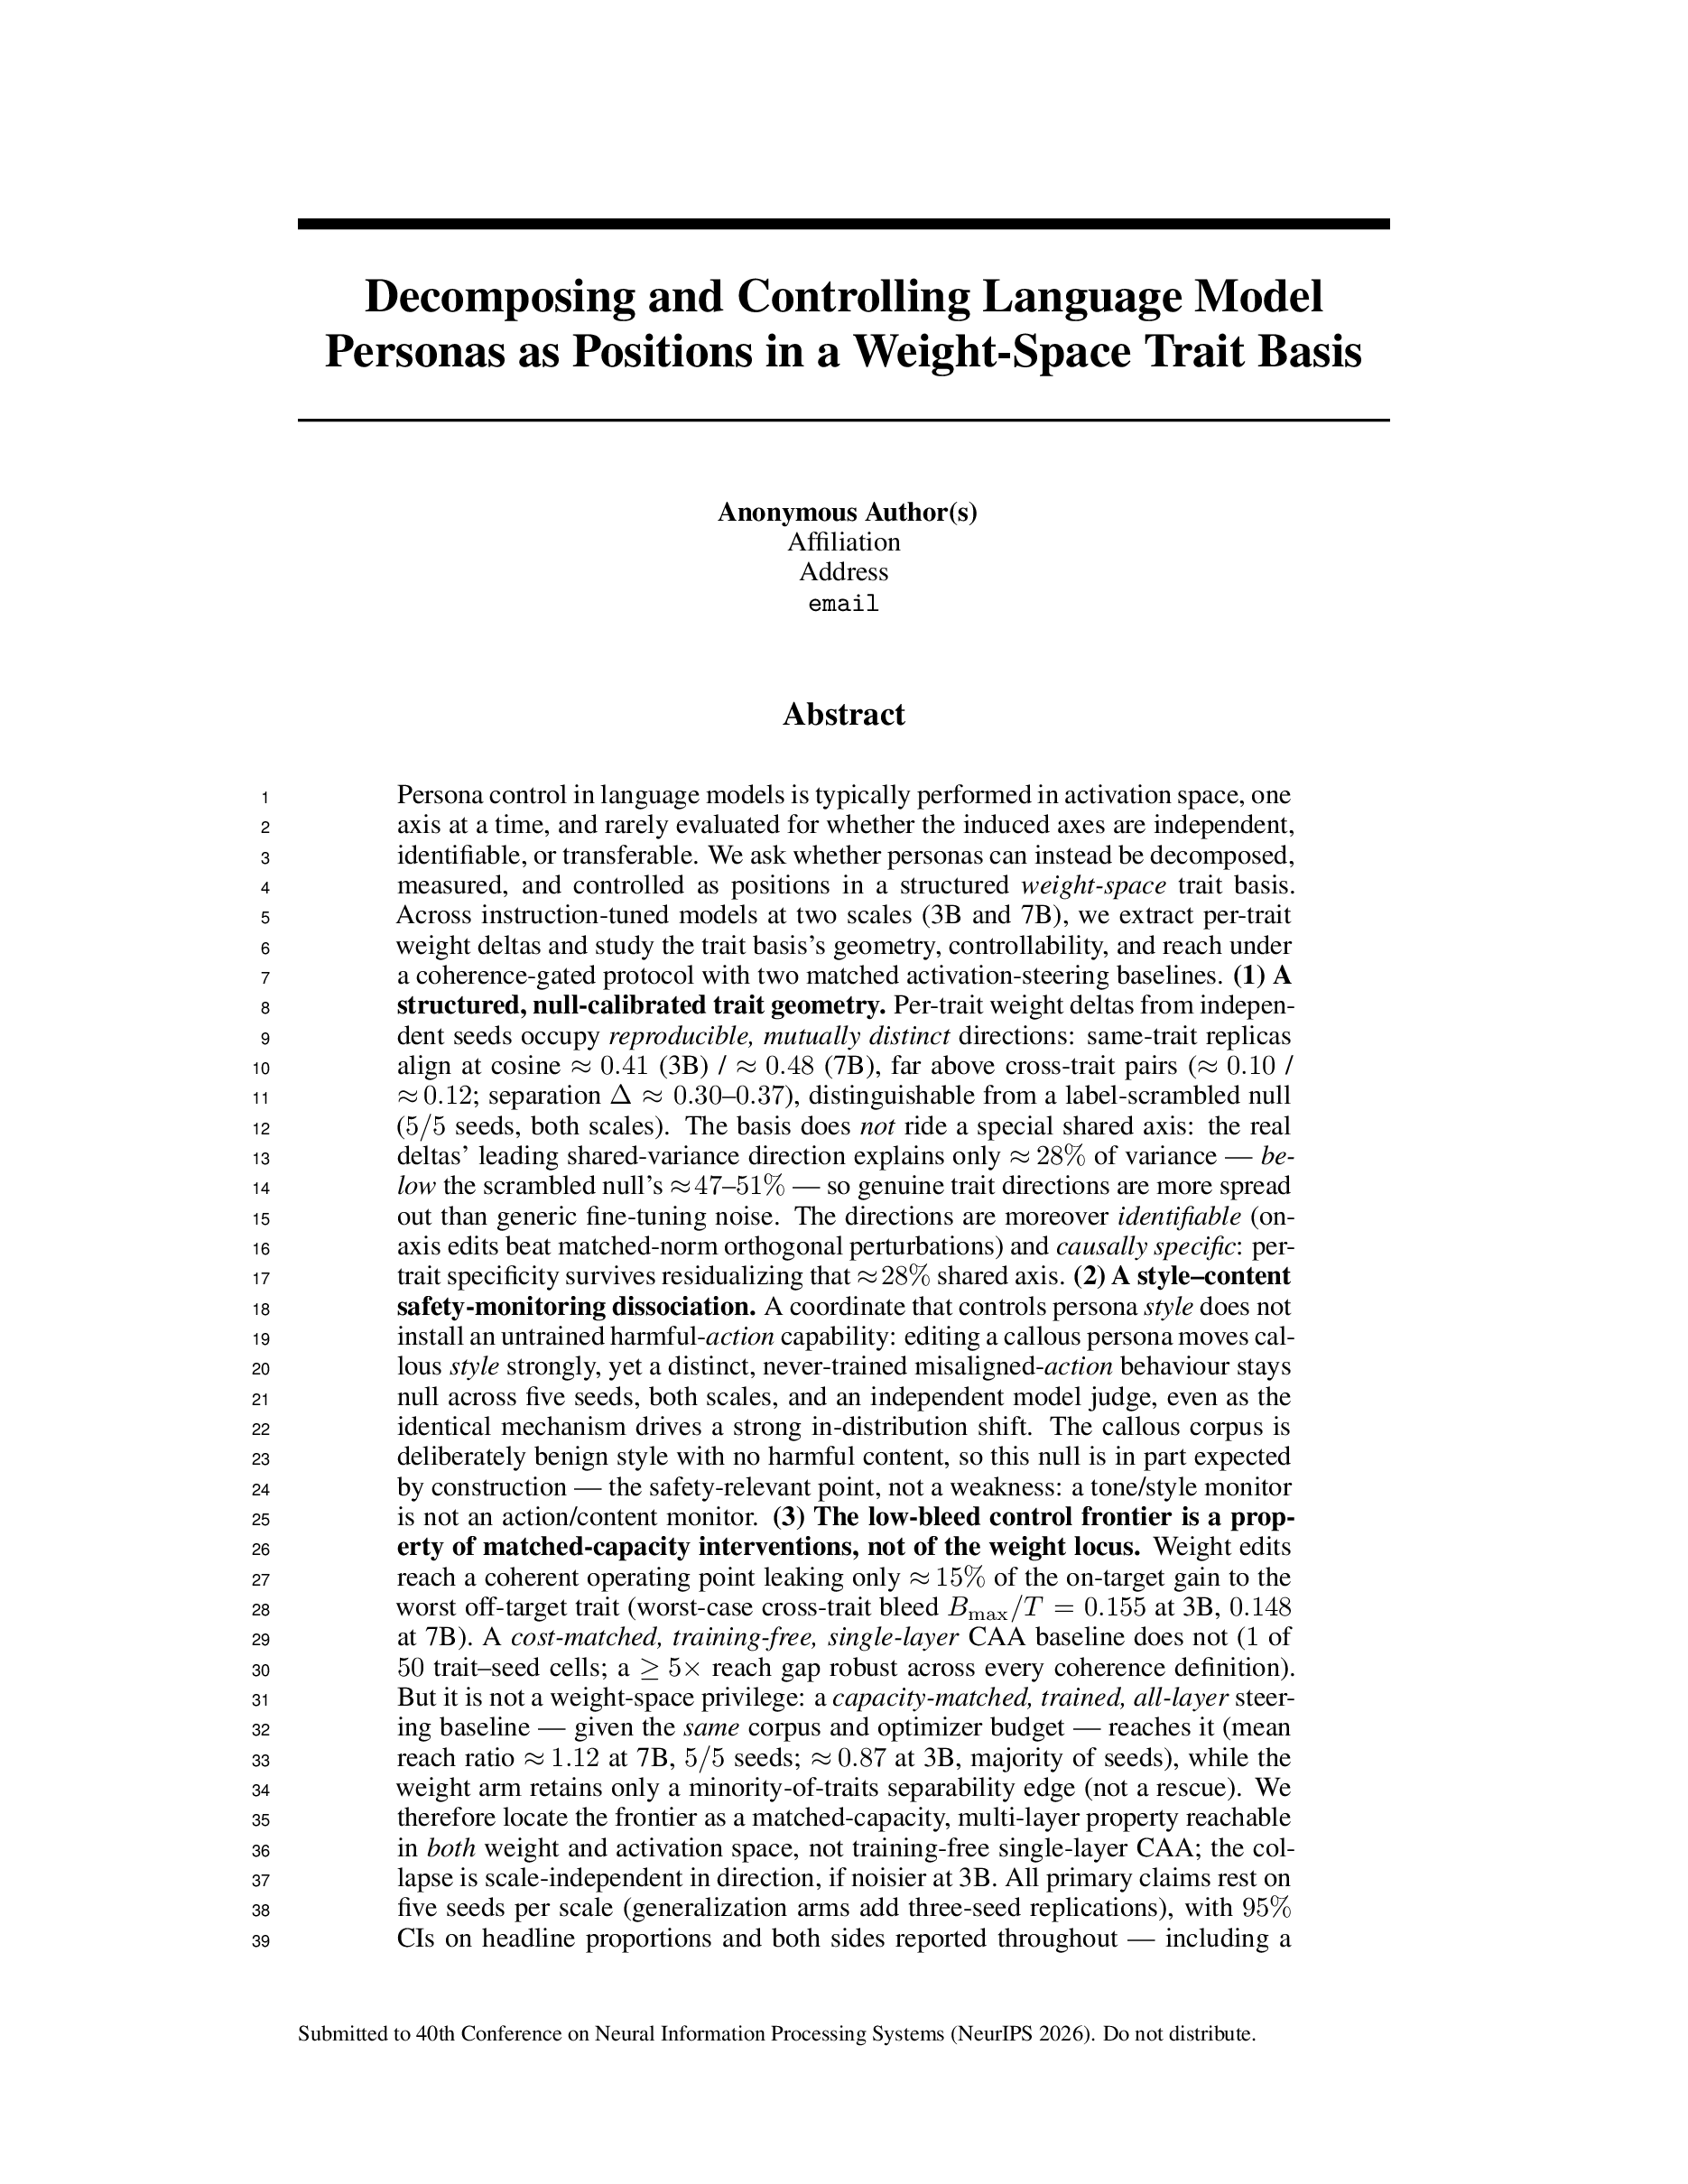
\includegraphics[width=4.03cm,trim={55bp 20bp 55bp 35bp},clip]{assets/personas-abstract-unedited.png}};
  \node[anchor=north west,inner sep=0pt]
    at (4.15,5.98) {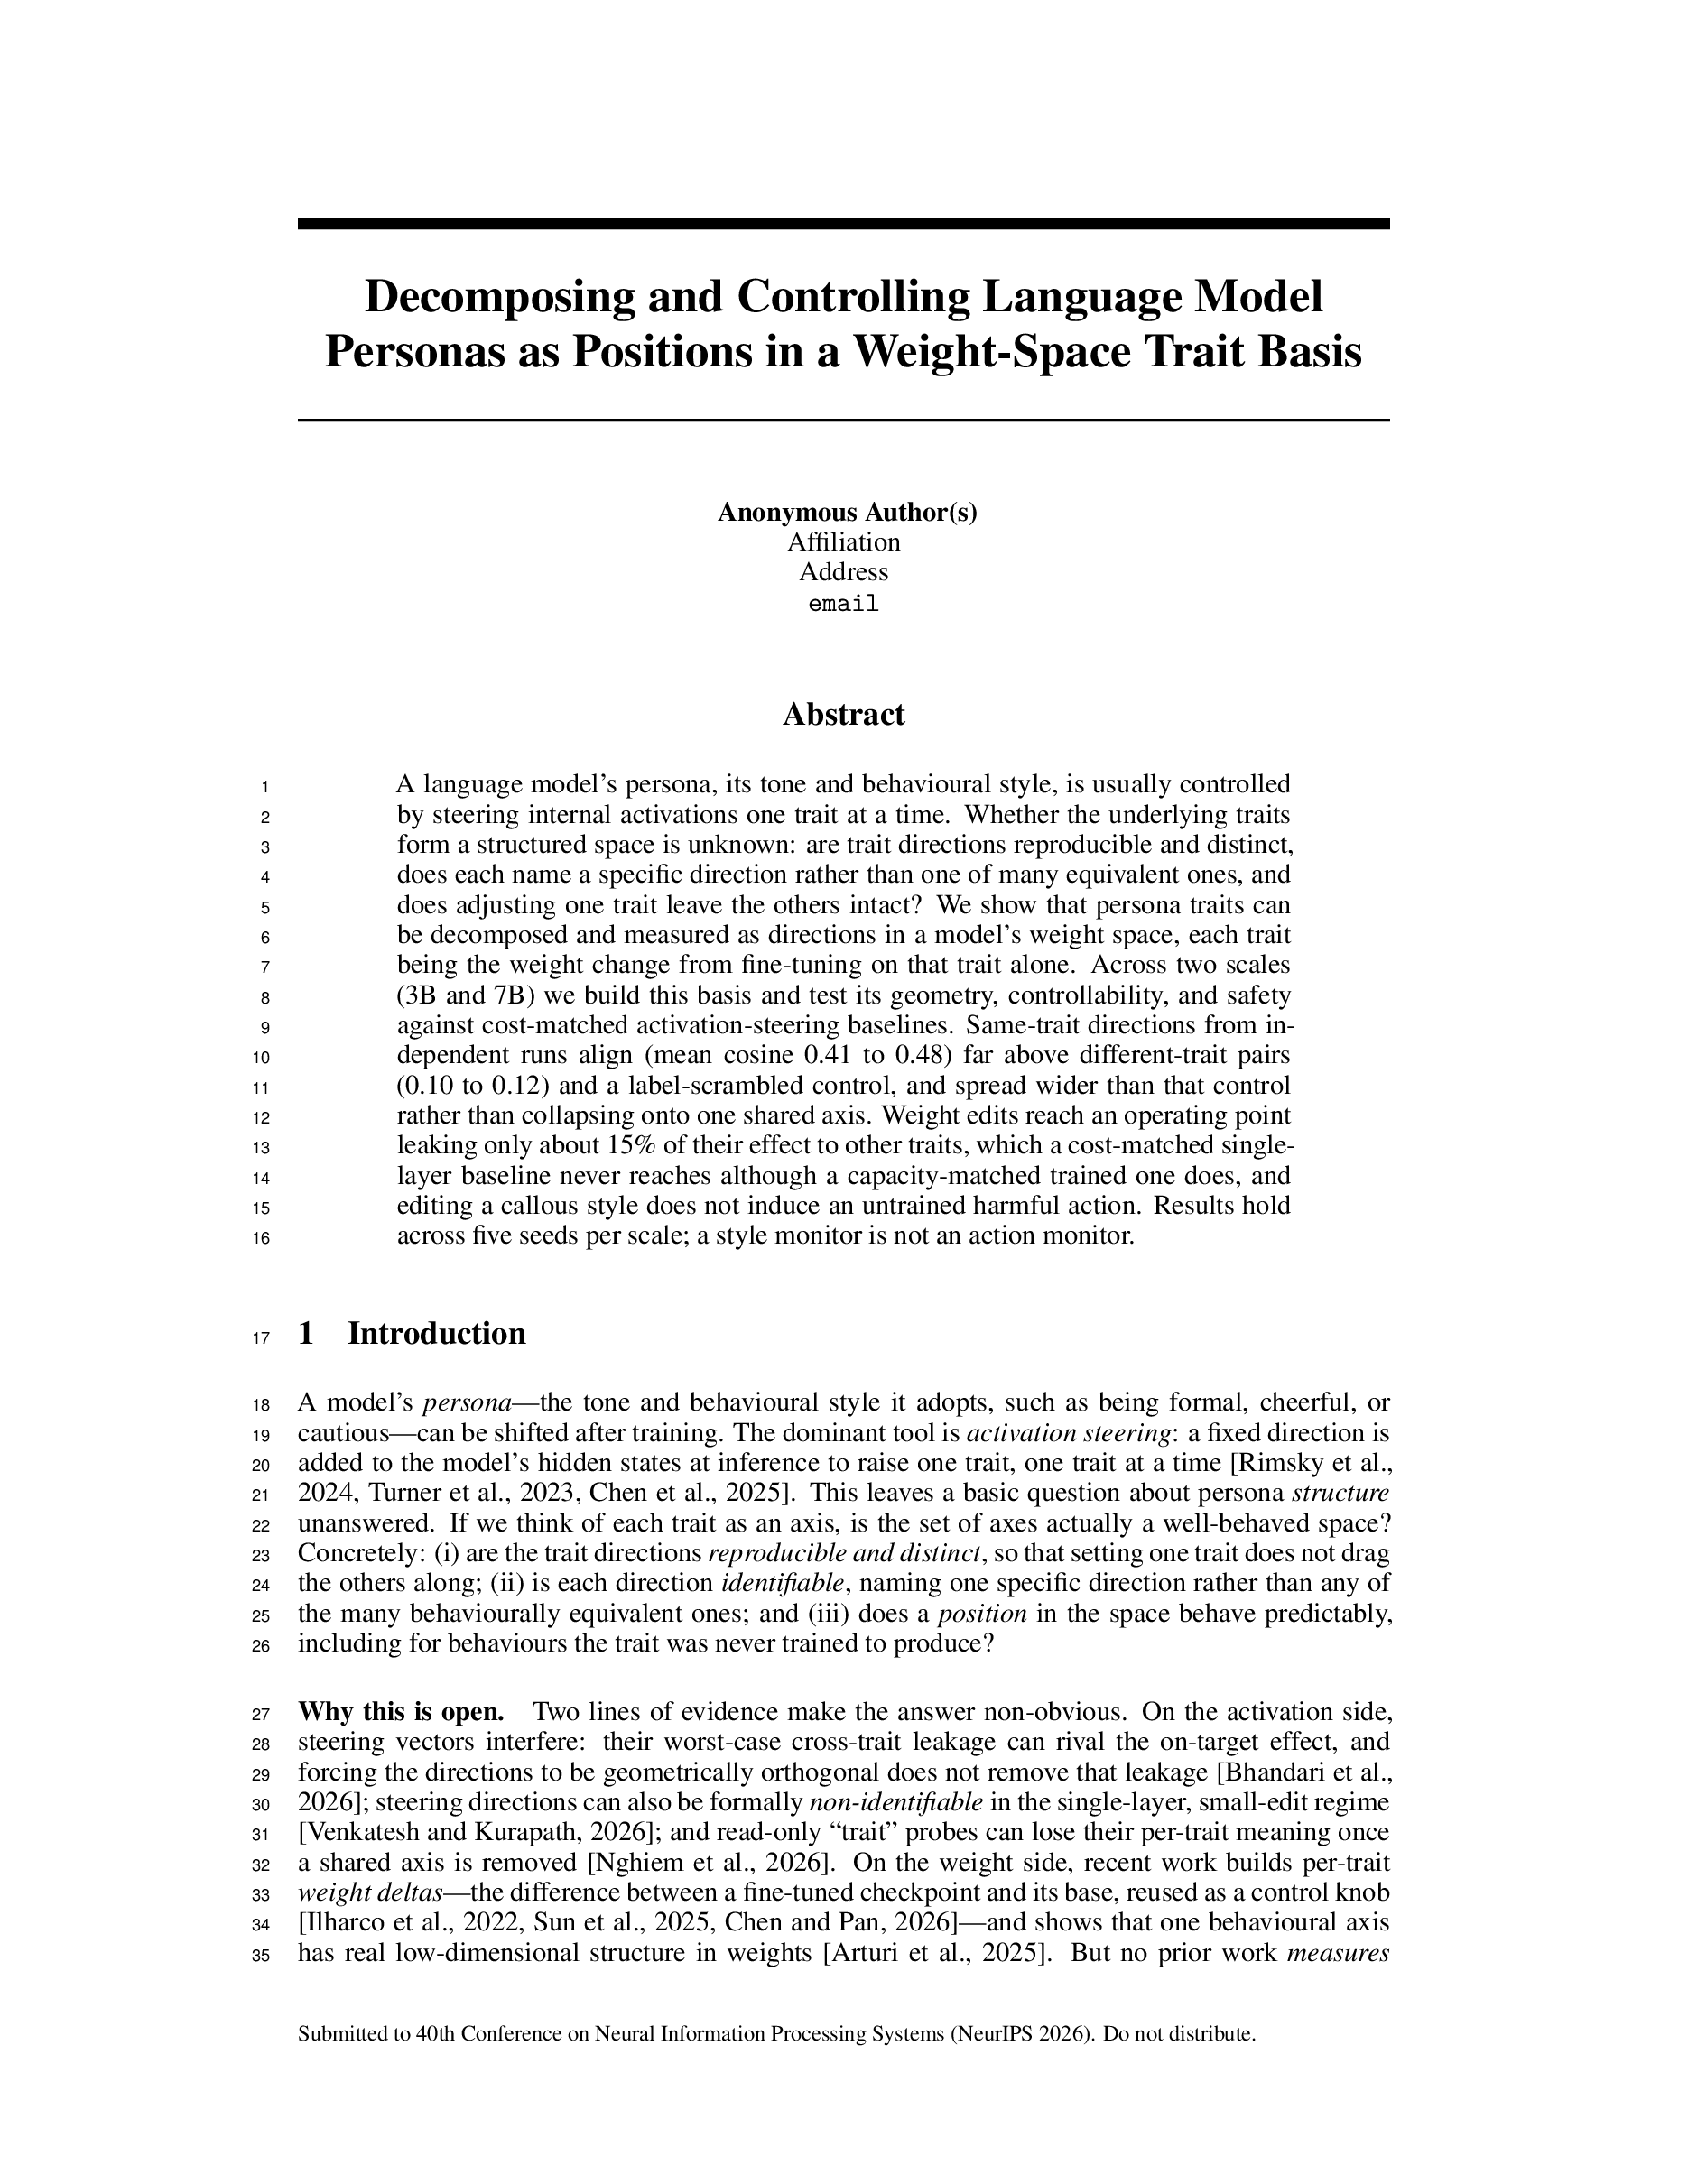
\includegraphics[width=4.03cm,trim={55bp 20bp 55bp 35bp},clip]{assets/personas-abstract-final.png}};
  \node[anchor=north west,inner sep=0pt]
    at (8.30,5.98) {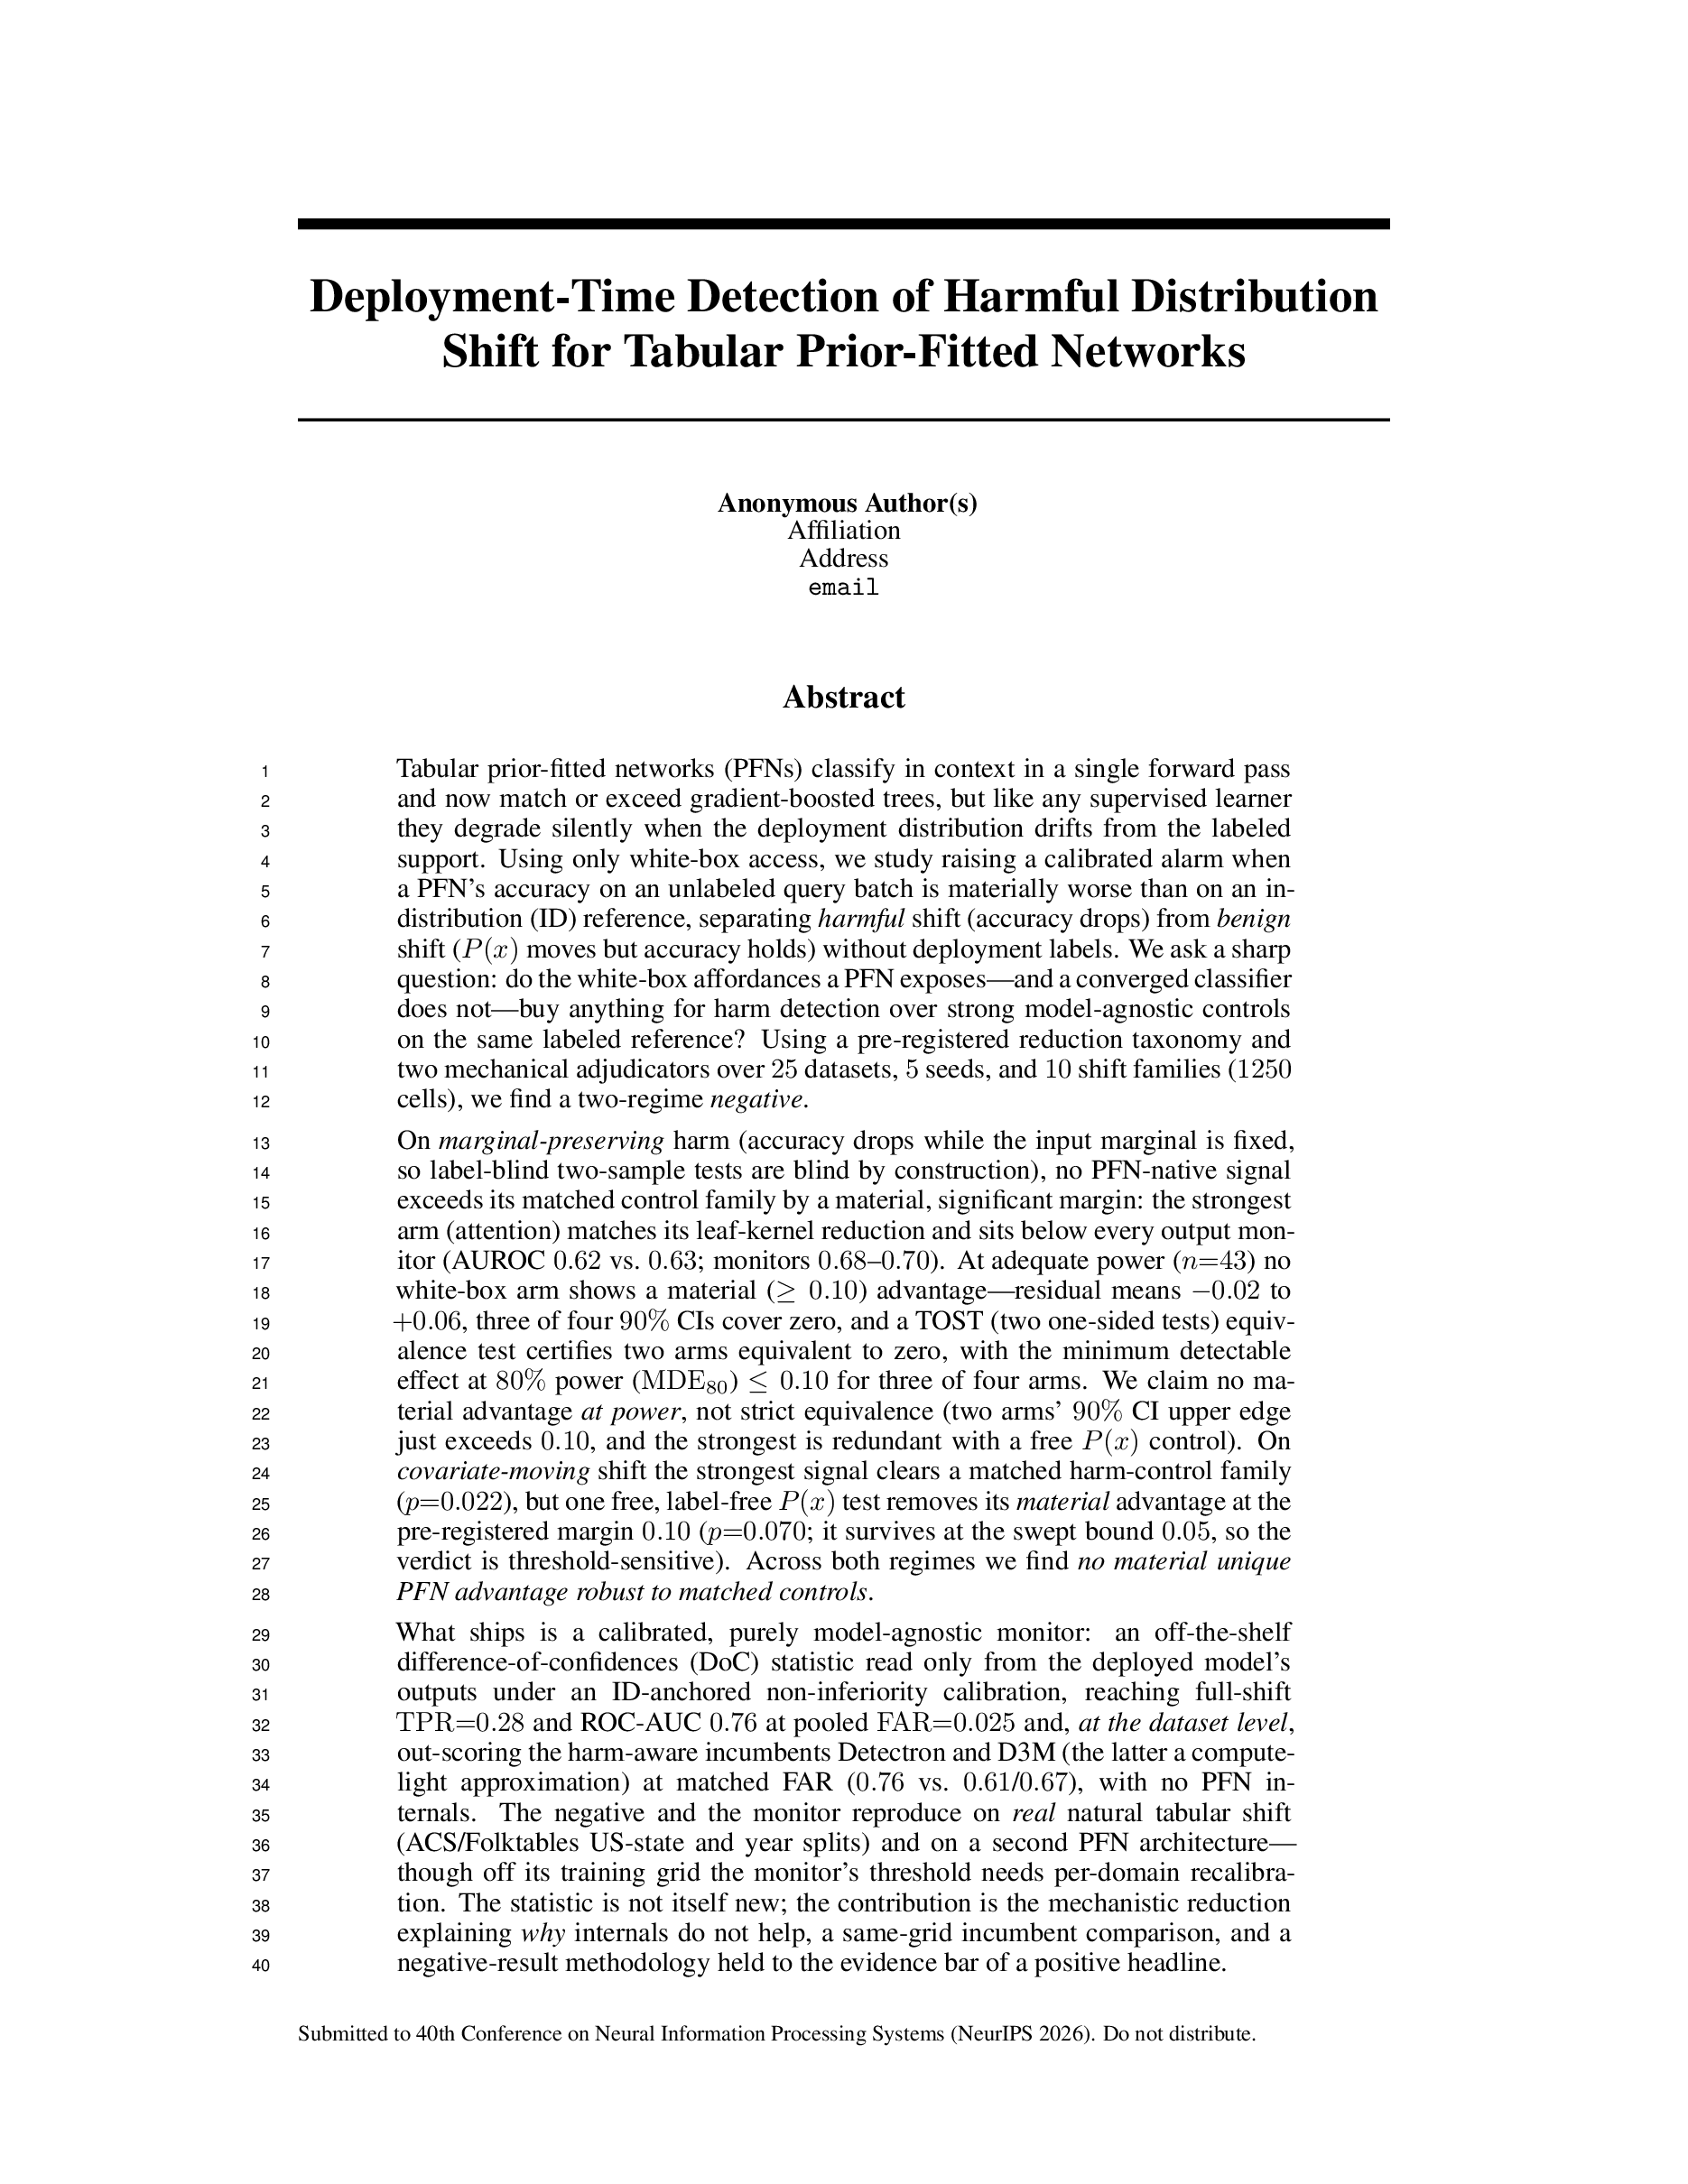
\includegraphics[width=4.03cm,trim={55bp 20bp 55bp 35bp},clip]{assets/tabpfn-abstract-unedited.png}};
  \node[anchor=north west,inner sep=0pt]
    at (12.45,5.98) {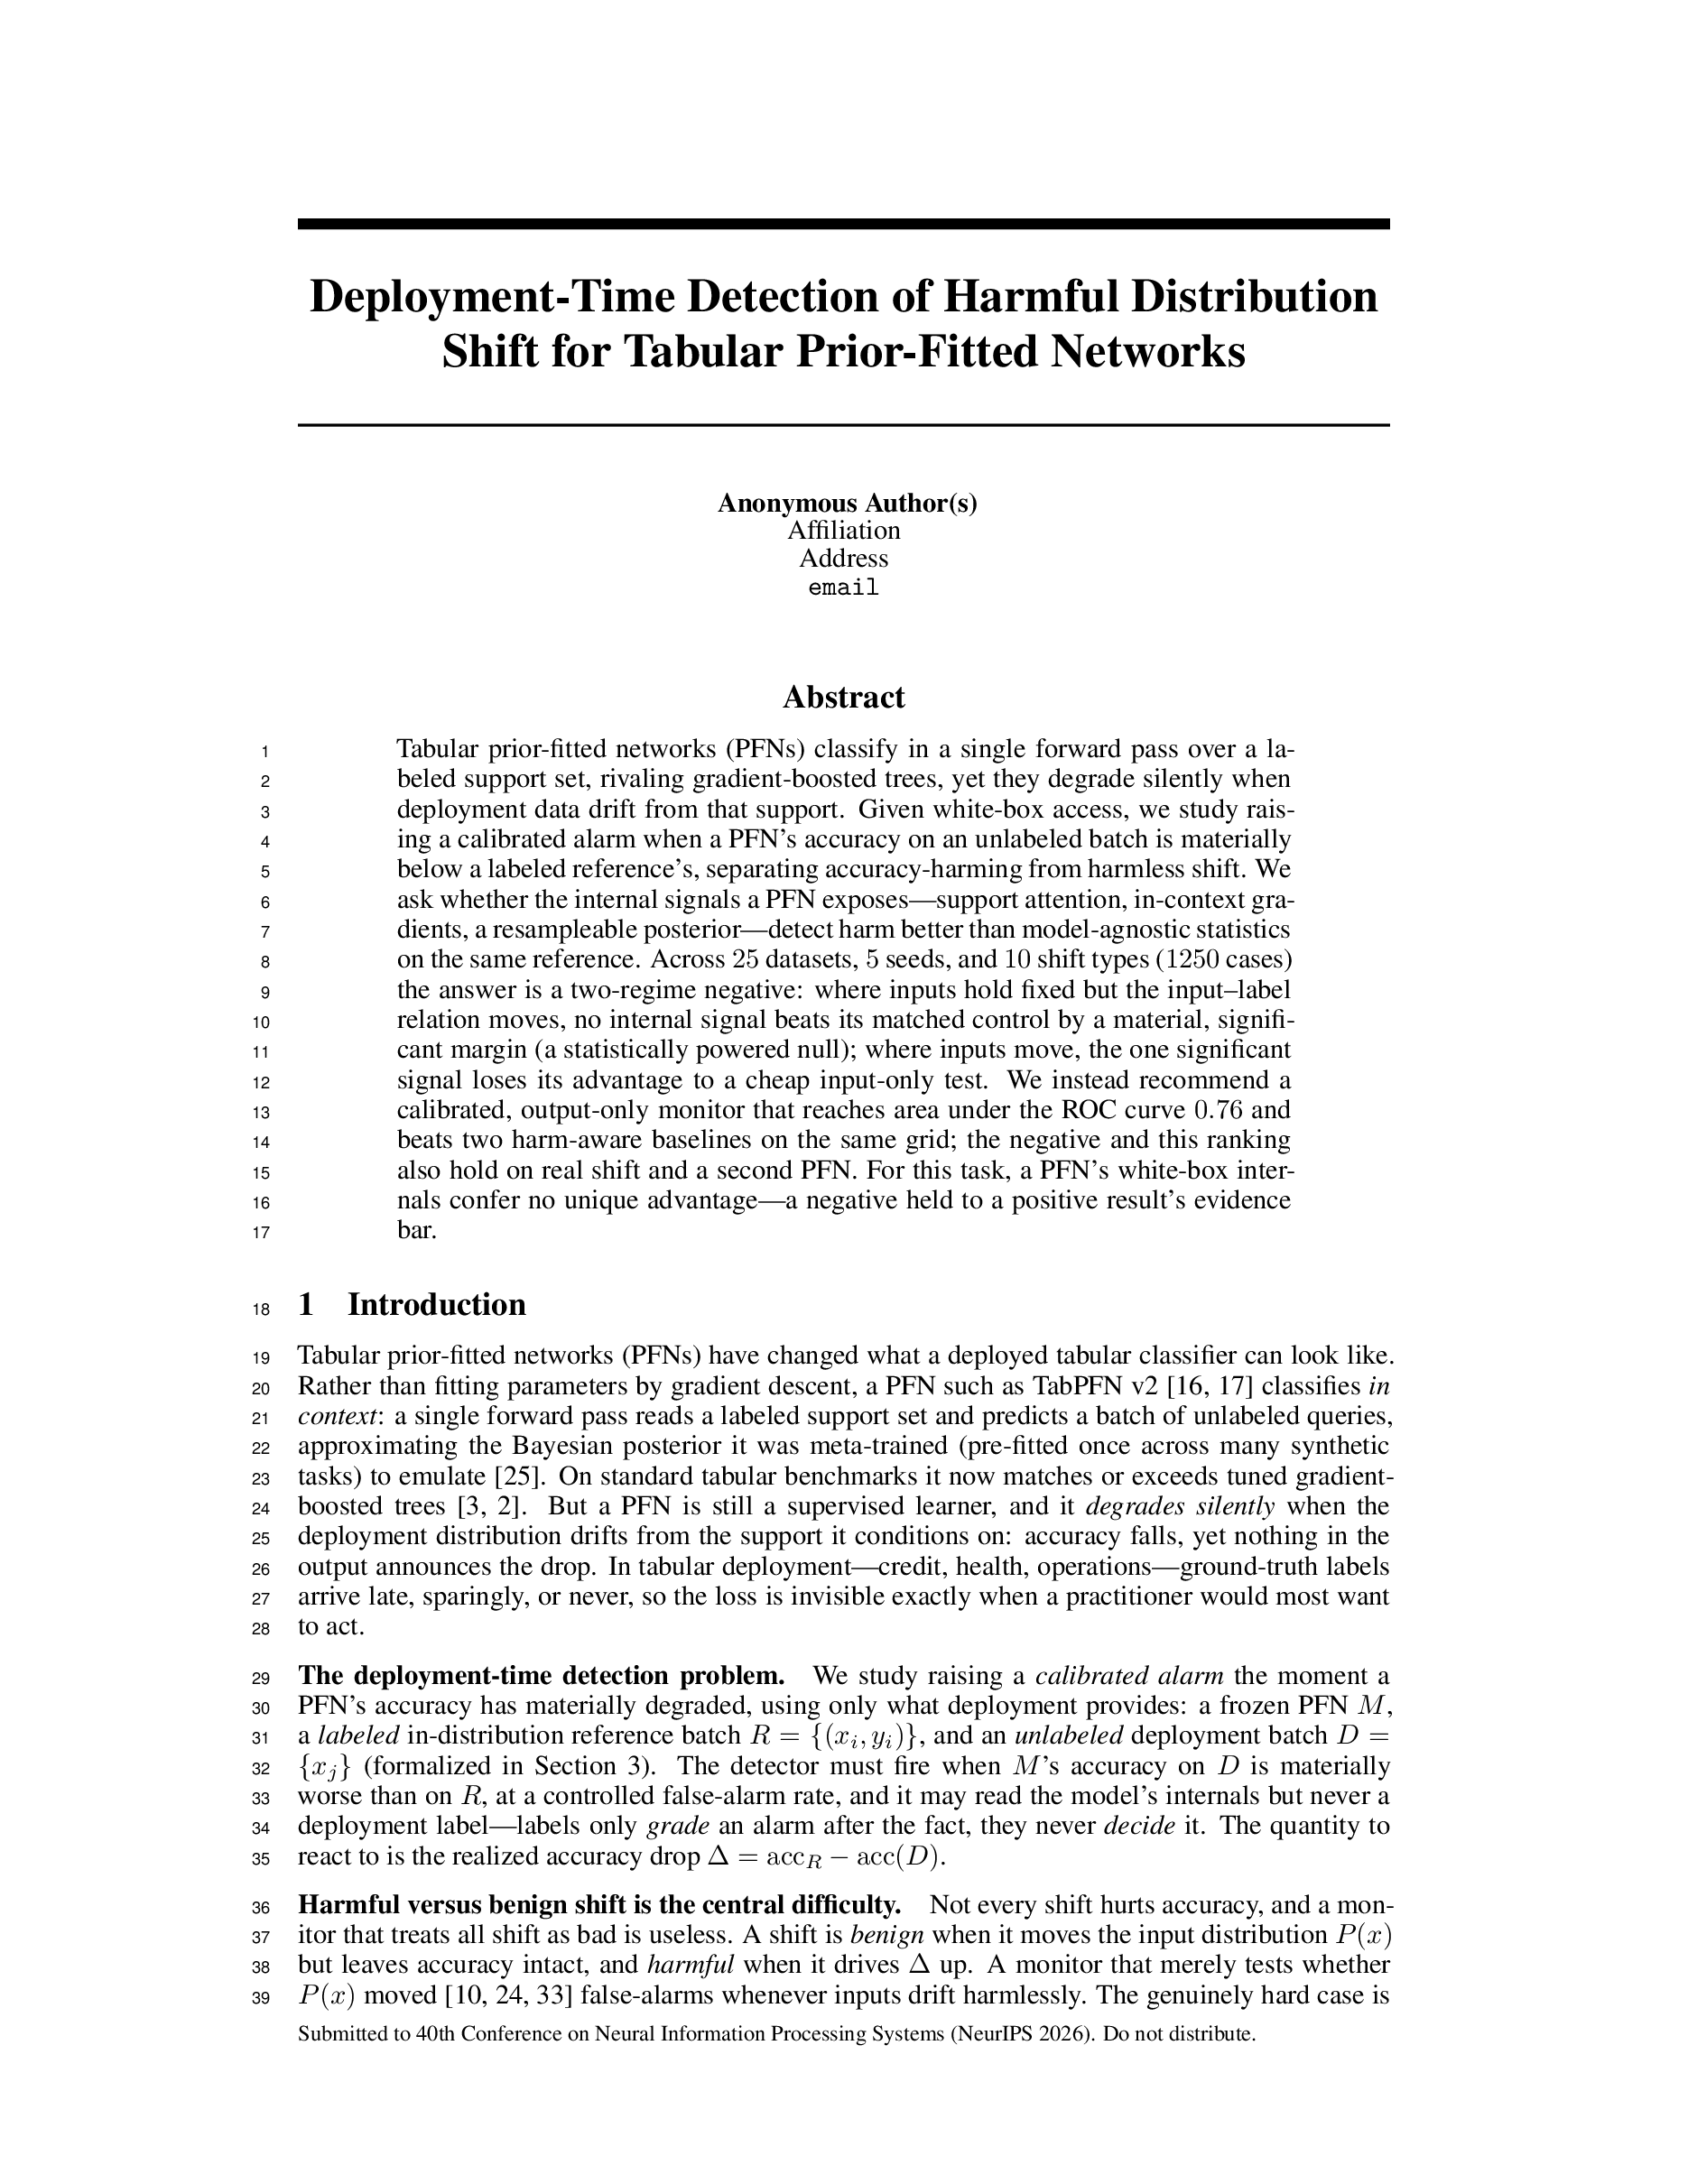
\includegraphics[width=4.03cm,trim={55bp 20bp 55bp 35bp},clip]{assets/tabpfn-abstract-final.png}};
\end{tikzpicture}

  \caption{Comparison of the submitted papers before and after a human
  intervention which instructed a final pass from the agent for readability.}
  \label{fig:readability-comparison}
\end{figure}

A majority of respondents thought the final paper would have obvious
misformatting (7 of 11).

\subsection{We found no significant reward hacking}

We reviewed the raw LLM calls and all of the code the agents committed. Our
review did not find any evidence of the agent reward hacking in the sense of hiding or misrepresenting
experiments or data to support a more compelling conclusion. In fact, we were
surprised that the trend was the opposite; the agents began with more
marketable claims and diligently retired them in favor of negative
results.\footnote{Some collaborators argued that prematurely coalescing on a
negative result was similar to reward hacking, but our definition would limit
reward hacking in this experiment to a paper which deceived the verifier into
giving a high score for a paper with a marketable, but ultimately unsupported,
result.} The agent also provided code to make sure every result in the paper
was reproducible, and developed a single script to reproduce all results,
though the repository was not well organized. Instead of clear, reusable
components, it comprised a sprawling set of folders, though this is also
common in academic research.

Our log analysis did note two other safety-relevant behaviors. First, in one of the runs, the agent committed an access token to the repository. Second, we found five instances of subagents hallucinating or misrepresenting results, but in each case, the orchestrator agent (which was specifically instructed to double-check their work) was able to uncover the issue, meaning none of them were present in the final draft.

Very few respondents expected the agent to take a catastrophic action (2 of
11). Less than half thought the agent would misreport or lie about the success
of an experiment (4 of 11). A majority thought the agent would p-hack or
cherry-pick the results (7 of 11).

\subsection{Higher reasoning effort improved the quality of results}

Before conducting the two experiments we discuss above, which used extra-high
reasoning, we conducted two dry runs on these same papers with Opus 4.8 without
reasoning. Those runs suffered from the same failure modes, but also suffered
from poor literature review and much worse writing quality. Instead of
conducting an in-depth literature review, the agents skimmed the literature.
They returned inscrutable papers within a few days rather than working closer
to the deadline.

We did not think the outputs were good enough to warrant external review from
the original authors of the papers. This shows that despite the weak performance
observed in our final experiments, more reasoning helped improve performance. We
tentatively think that more reasoning effort within model calls might improve
performance, but more wall-clock time or resources would not significantly
change the results. In dry runs, the agents often timed out when using max
reasoning, so we used extra-high reasoning for our final runs.

\subsection{We tried to use frontier models to improve the harness, with
limited success}

After our initial pilots, in addition to increasing reasoning effort, we
conducted a comprehensive manual log analysis ourselves, and then tasked
Claude Fable 5 with improving our scaffold based on the failures observed in
the pilots.\footnote{We used Claude Code with Fable 5 in goal mode and the
``ultracode'' setting. We asked it to take the results from our pilot
experiments, a telemetry file with the full agent log, and the OpenClaw
documentation and edit the scaffold to ensure that the failure modes we
observed would not be repeated.} Many of the same failure modes we identify
throughout our experiments also appeared in this scaffold improvement process:
the agent assigned disproportionate weight to a single $n=1$ sample, making broad changes to the scaffold and idiosyncratically swapping rules and heuristics throughout, none of which seemed to address the fundamental problems we identified.

\section{Log analysis reveals five failure modes}
\label{sec:failure-modes}

Our experiments provide some evidence that frontier AI agents are not capable
of autonomously producing machine learning research papers at the caliber of
top conference submissions with nearly unconstrained inference-time compute,
large external resource budgets, and general-purpose scaffolds.

They do suggest current frontier AI agents can do the engineering work that is
a prerequisite for autonomous AI R\&D. Without any human intervention, they
are capable of navigating each of the environments necessary to, in principle,
make contributions to AI science. For example, in both of our experiments, the
agents debugged and managed GPU resources and ran compute-intensive
experiments.

Our analysis of the agents' logs identifies five primary causes of failure.
First, they lacked judgment to identify when to incorporate substantive feedback and what aspects of the research question would make for compelling research outputs. Second, they could not creatively solve shortcomings in the research design to address negative feedback from AI reviewers. While our experts judged the initial hypotheses generated by the agents as cogent and interesting, as those hypotheses were falsified, the agents struggled to pivot to new and creative
approaches. Third, they could not effectively backtrack from failing
approaches. They regularly made small pivots to their approach, but did not
fundamentally rethink their approach or try new approaches from scratch.
Fourth, they lacked context awareness. They were unable to effectively use
resources given to them, such as VMs and API limits, and they could not keep
track of the deadline. Finally, they suffered from instruction drift. Even
when we instructed agents to carry out certain tasks, they suffered from
context rot during compaction and were unable to effectively use these
instructions. 

\subsection{Lack of judgment about the bar for high-quality research}

The goal established for the agent was to write a NeurIPS-quality paper on a
well-defined research problem. But the agents' planning and execution did not
indicate a clear ``model'' of these expectations. Both expert reviews
highlighted major issues of data selection: in both experiments, the agents
only utilized underpowered synthetic datasets or hand-picked examples that
were not very broad.\footnote{In the TabPFN paper, the agent did work with real datasets from OpenML, but the shifts in the data were synthetic. The agent only used real-world shifted datasets for a set of final experiments to corroborate its original findings.} Our analysis supports the view that the agents coalesced
around a research direction well before it was warranted from the evidence.

The agents' internal review process, despite never returning an accept, was
inflated relative to our expert human reviewers: it mostly returned ``Weak
Reject'' for papers that our experts unambiguously rejected. Had these reviews
been better calibrated, the agents might have recognized that they needed to
shift their approach rather than making incremental revisions.

Limitations in the calibration of AI agents have been documented elsewhere.
In our own experiments testing AI agent reliability on standard benchmarks,
we found that current frontier models remain poor discriminators of task
success, even as their accuracy has increased. A similar open-ended
post-training experiment conducted by the AI Village also highlighted poor
data selection as a main failure mode~\citep{tekofsky2026finetuneleader}.


\subsection{Lack of creative problem solving}

The agents surfaced many creative hypotheses at the start of the project. As
we discussed earlier, both authors judged the initial hypotheses reasonable
and interesting, and noted that they resembled their own early approaches to
the problem. However, when agents' small-scale synthetic experiments and AI
reviews showed that the results were not strong enough, the task shifted from
proposing ideas to creative problem solving, such as developing an alternative framing of the question, redesigning an underpowered experiment, or constructing a stronger test of the same hypothesis. Here, the agents suffered from a lack of creative problem-solving ability.

We instructed the agents to use several sources of AI feedback throughout the
project, including a review subagent and external AI reviewing tools. This
setup worked as designed; the AI reviews surfaced many of the same failure
modes as our expert reviews did. But the agents' responses did not address the central critiques: they typically focused on minor comments, added qualifications, or adopted less ambitious hypotheses. This produced papers with
extremely thorough negative findings rather than papers with new ideas. In a
progress report, David Africa observed that the agent's hypotheses ``grew
narrower and less interesting as it discarded each one.'' We suspect that even
if we had extended the wall-clock time by multiple weeks, the agents would
have been unlikely to pivot toward a positive result, even if one could have
been supported by the data.

This failure is related to a well-known weakness of LLMs: failing to question the
premise of a request. It is perhaps best illustrated by the fact that LLMs
still have not saturated ``trick question'' multiple-choice benchmarks like
SimpleBench~\citep{epochsimplebench}, even as they saturate much more technically challenging
benchmarks in domains like software engineering.

Note that our coauthors disagree about the root cause for this failure;
candidates include a lack of creativity, epistemic lock-in, myopia, and
functional fixedness. We use ``creative problem solving'' because it describes
what the task required, while the other terms describe mechanisms for how the
agent failed; however, we explicitly surface the disagreement since it is an
example of the kind of subjective decisions that open-ended shadow evaluations
involve.

\subsection{Lack of effective backtracking}

Even without a new idea, a researcher can recognize that an approach is unproductive, discard the work, and return to exploration. The agents backtracked locally, rerunning experiments and adding robustness checks in response to critique. But they never backtracked at the level of the project. Despite AI self-reviews
consistently returning negative verdicts, neither agent responded by
abandoning its approach and restarting. In the TabPFN run, the agent instead
reframed the goal: after its early detector attempts failed, it argued that no
such detector could exist and wrote a negative-results paper. Our design
required the agent to produce a paper and offered no option to abstain, which
may have led the agent to write a negative-results paper. But a human
researcher in the same position might have backtracked much earlier and more
effectively while sufficient time and budget remained to pursue an alternative
approach.

This was not because of a scaffold limitation; agents had the tools to
backtrack within the scaffold. They could spawn subagents with clean context,
without information about failing approaches, and they used subagents
routinely for other purposes. However, they rarely used them to
restart.\footnote{In the TabPFN run, the agent considered six distinct
approaches, but falsified each of them within the first fourteen hours. Despite 110
hours remaining against the original deadline, the agent never revised its
solution approach after this point.}

\subsection{Lack of context awareness}

The agents left most of their budgets unused. Each agent balanced three
budgets: its own tokens, external compute, and the clock. It could check all
three at any moment.\footnote{The agent records this in the agent log each time
it checks, so we can confirm that this tool was frequently used throughout the
trajectory.} Both runs still ended with less than half the API budget spent.
One agent declared the project complete seven hours before the deadline,
shortly after its own reviewer returned another reject. A human researcher in
that position might have spent every remaining hour improving the paper.
The complete time, API, and GPU-compute trajectories are summarized in
\Cref{fig:resource-use}.


This failure appears in other evaluations too. As one example, the
PostTrainBench leaderboard~\citep{posttrainbenchleaderboard} results for GPT-5.5 have an explicit note saying
that ``the agent was manually prompted to continue each time it stopped before
the time budget expired.'' We think this failure results from the lack of
calibration about what agents can do in hours of time. They are trained on
human data but have very different affordances. Unlike a person, an agent can
read and edit the paper hundreds of times in the span of a few hours, but it
does not seem to recognize this.


\subsection{Instruction drift}

The agents increasingly failed to follow explicit instructions over the course of the run. We gave each agent one paid credit for refine.ink, the strongest AI review tool available to it. The agents only used it in one of two final runs. We set
limits on paper length and abstract length. Both final papers exceeded them.
We set rules for how much time to spend on exploration. The agents acknowledged
these rules early in the run and then ignored them. We think this failure
generalizes beyond our setup. On a multi-day project, the agent needs to
actively manage its context window to retain what information is considered
important; our results point to agents not yet being proficient at this task.

%\FloatBarrier
